\documentclass[a4paper, 11pt]{article}
\usepackage[polish]{babel}
\usepackage[T1]{fontenc}
\usepackage[utf8]{inputenc}
\usepackage{hyperref}
\usepackage{array}
\usepackage{amssymb}
\usepackage{amsmath}
\hypersetup{
    colorlinks,
    citecolor=black,
    filecolor=black,
    linkcolor=black,
    urlcolor=black
}
\usepackage{graphicx}

\usepackage{tikz}
\usetikzlibrary{fit,arrows,matrix,positioning, calc, shapes.gates.logic.IEC, shapes.gates.logic.US,arrows,arrows.meta}
\tikzstyle{branch}=[fill,shape=circle,minimum size=3pt,inner sep=0pt]

\title{%
        \vspace{-3.5cm}
       \large Sprawozdanie Laboratorium PTC \\
       \huge Układy Sekwencyjne 1}

\author{Stanisław Fiedler 160250, L1}
\date{LAB 3, 4 listopada 2024}

\begin{document}

\maketitle
%\tableofcontents

Zmodyfikuj licznik z zadania 1, tak aby liczył w kodzie Graya.

\section{Graf Przejść}\label{sec:graf} % (fold)

\begin{center}
	\begin{tikzpicture}
		\node[shape=circle,draw=black] (s0) at (0,0) {$S_0$};
		\node[shape=circle,draw=black] (s1) at (3,0) {$S_1$};
		\node[shape=circle,draw=black] (s2) at (6,0) {$S_2$};
		\node[shape=circle,draw=black] (s3) at (9,0) {$S_3$};

		\begin{scope}[>={Stealth[black, scale=1.5]},
			every node/.style={fill=white}]

			\path [->] (s3) edge[bend left=30] node {0} (s0);
			\path [->] (s0) edge[bend left=30] node {1} (s3);
			\path [->] (s0) edge[bend left=20] node {0} (s1);
			\path [->] (s1) edge[bend left=20] node {0} (s2);
			\path [->] (s2) edge[bend left=20] node {0} (s3);
			\path [->] (s3) edge[bend left=20] node {1} (s2);
			\path [->] (s2) edge[bend left=20] node {1} (s1);
			\path [->] (s1) edge[bend left=20] node {1} (s0);

		\end{scope}

	\end{tikzpicture}
\end{center}

% section  (end)

\section{Tabica przejść oraz zakodowana tablica przejść}\label{sec:tablica} % (fold)
\begin{center}
	\begin{tabular}{ c | c c }
		      & 0     & 1     \\
		\hline\hline
		$S_0$ & $S_1$ & $S_3$ \\
		$S_1$ & $S_2$ & $S_0$ \\
		$S_2$ & $S_3$ & $S_1$ \\
		$S_3$ & $S_0$ & $S_2$ \\
	\end{tabular}\hspace{1cm}
	\begin{tabular}{ c | c c }
		     & 0    & 1    \\
		\hline\hline
		$00$ & $01$ & $10$ \\
		$01$ & $11$ & $00$ \\
		$11$ & $10$ & $01$ \\
		$10$ & $00$ & $11$ \\
	\end{tabular}
\end{center}

% section  (end)

\section{Fukcje wzbudzeń}\label{sec:} % (fold)

\begin{center}

	\begin{tabular}{ | c | c | c || c | c | }
		\hline
		X & $Q_1$ & $Q_0$ & $D_1$ & $D_0$ \\
		\hline\hline
		0 & 0     & 0     & 0     & 1     \\
		0 & 0     & 1     & 1     & 1     \\
		0 & 1     & 0     & 0     & 0     \\
		0 & 1     & 1     & 1     & 0     \\
		1 & 0     & 0     & 1     & 0     \\
		1 & 0     & 1     & 0     & 0     \\
		1 & 1     & 0     & 1     & 1     \\
		1 & 1     & 1     & 0     & 1     \\
		\hline
	\end{tabular}

\end{center}

\begin{center}
	\Large $D_{1}$\\
	\begin{tikzpicture}
		\matrix (Y1) [matrix of math nodes, nodes in empty cells, nodes={minimum height=1cm, minimum width=1cm, anchor=center}, column 1/.style={nodes={minimum height=1cm, minimum width=2cm, anchor=center}}] (m)
		{
				{} & 00 & 01 & 11 & 10 \\
				0             & 0  & 1  & 1  & 0  \\
				1             & 1  & 0  & 0  & 1  \\
			};
		\draw[double distance=2pt] (m-1-2.north west) -- (m-3-2.south west);
		\draw[double distance=2pt] (m-1-1.south west) -- (m-1-5.south east);;
		\node[fit={(m-2-3.north west) (m-2-4.south east)},
			thick, inner sep=0pt, rounded corners=1mm,
			draw=green ]{};
		\node[fit={(m-3-5.north west) (m-3-5.south east)},
			thick, inner sep=0pt, rounded corners=1mm,
			draw=blue ]{};
		\node[fit={(m-3-2.north west) (m-3-2.south east)},
			thick, inner sep=0pt, rounded corners=1mm,
			draw=blue ]{};
		\draw (m-1-1.north west) -- (m-1-1.south east);
		\node[anchor=south west, font=\Large] at ($(m-1-1.center) + (-0.5,0.0)$) {$Q_{1}Q_{0}$};
		\node[anchor=north east, font=\Large] at ($(m-1-1.center) + (-0.2,0.2)$) {$X$};
	\end{tikzpicture}
	\raisebox{1cm}{ \large $ \quad D_1 = \bar{X}Q_0 + X\bar{Q_0} $ }
\end{center}

\begin{center}
	\Large $D_{0}$\\
	\begin{tikzpicture}
		\matrix (Y1) [matrix of math nodes, nodes in empty cells, nodes={minimum height=1cm, minimum width=1cm, anchor=center}, column 1/.style={nodes={minimum height=1cm, minimum width=2cm, anchor=center}}] (m)
		{
				{} & 00 & 01 & 11 & 10 \\
				0             & 1  & 1  & 0  & 0  \\
				1             & 0  & 0  & 1  & 1  \\
			};
		\draw[double distance=2pt] (m-1-2.north west) -- (m-3-2.south west);
		\draw[double distance=2pt] (m-1-1.south west) -- (m-1-5.south east);;
		\node[fit={(m-2-2.north west) (m-2-3.south east)},
			thick, inner sep=0pt, rounded corners=1mm,
			draw=green ]{};
		\node[fit={(m-3-4.north west) (m-3-5.south east)},
			thick, inner sep=0pt, rounded corners=1mm,
			draw=blue ]{};
		\draw (m-1-1.north west) -- (m-1-1.south east);
		\node[anchor=south west, font=\Large] at ($(m-1-1.center) + (-0.5,0.0)$) {$Q_{1}Q_{0}$};
		\node[anchor=north east, font=\Large] at ($(m-1-1.center) + (-0.2,0.2)$) {$X$};
	\end{tikzpicture}
	\raisebox{1cm}{ \large $ \quad D_0 = \bar{X}\bar{Q_1} + XQ_1 $}
\end{center}
% section  (end)

\section{Symulacja Logisim}\label{sec:symulacja_logisim} % (fold)

\begin{center}
	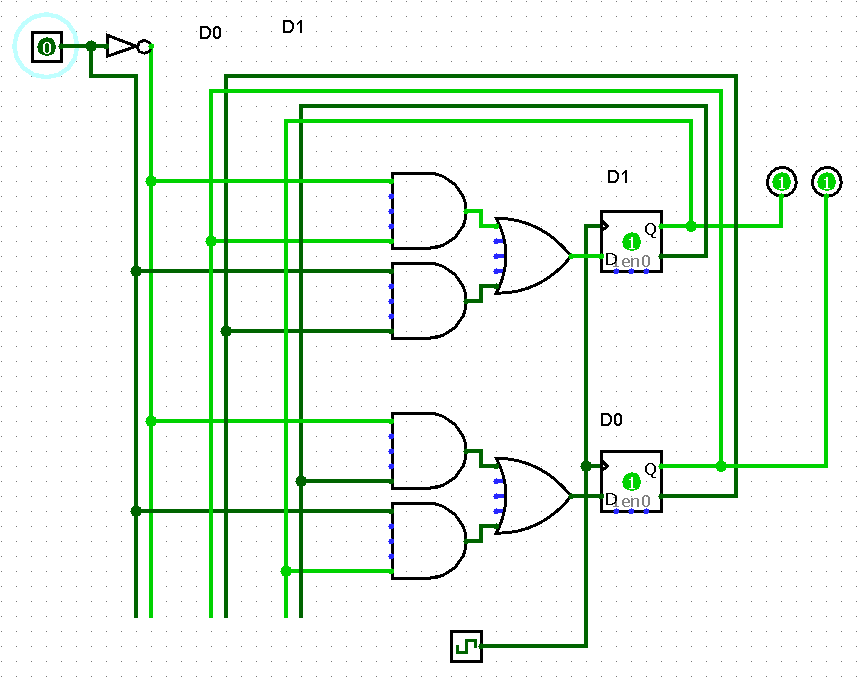
\includegraphics[scale=0.6]{images/ptclab3.png}
\end{center}

% section Symulacja Logisim (end)

\end{document}
